\documentclass[journal]{IEEEtran}
\usepackage[T1]{fontenc}
\usepackage{lmodern,amsmath,amssymb,graphicx,booktabs}
\usepackage[hidelinks]{hyperref}
\usepackage{url}
\DeclareMathOperator{\tr}{tr}
\DeclareMathOperator{\diag}{diag}
\DeclareMathOperator{\vecop}{vec}
\DeclareMathOperator{\unvec}{unvec}
\DeclareMathOperator{\Herm}{Herm}
\newcommand{\Hh}{^{\mathsf H}}
\newcommand{\F}{_{\mathrm F}}
\newcommand{\E}{\mathbb E}
\newcommand{\C}{\mathbb C}
\newcommand{\sn}{\operatorname{SINR}}
\newcommand{\norm}[1]{\lVert #1\rVert}
\title{Clutter-Aware Wideband ISAC Beamforming via Dual-Priced Directions and Power Allocation}
\author{Muneef Mohammed}
\begin{document}
\maketitle
\setlength{\abovedisplayskip}{7pt plus 2pt minus 2pt}
\setlength{\belowdisplayskip}{7pt plus 2pt minus 2pt}
\setlength{\jot}{2pt}
\begin{abstract}
A transmit beam that illuminates a sensing target can also increase the clutter power at the receiver. In a multiuser downlink, the same beam changes the interference at each user. We exploit the linear dependence of cold-clutter covariance on transmit covariance to design a wideband transceiver under per-user signal-to-interference-plus-noise requirements. With fixed distortionless receivers, power allocation over user-tagged beam directions is a linear fractional program. An equivalent linear program and its dual identify new directions by Hermitian eigenvalue problems and bound the loss due to restricting the direction set. We derive conditions under which recovering physical streams preserves communication feasibility. In a 32-tone MATLAB benchmark, the deterministic pricing solver with a fifteen-allocation budget returned feasible beams in all 72 scene--condition pairs. Across three operating conditions, median paired speedups over alternating semidefinite optimization ranged from 33 to 48, with median sensing shortfalls of 0.018--0.124 dB. A one-sided 0.1-dB target was attained on 38 of 70 pairs with feasible reference beams. In a separate 72-case ablation, joint clutter-aware design gained a paired median of 2.19 dB over adapting the receiver alone and 4.69 dB over a feasible zero-forcing control. We also test two uses of learning. Learned transmit proposals yielded little change after exact allocation. An eight-layer learned power update reduced the isolated first-allocation median objective gap from 0.544 to 0.055 dB relative to tuned tied steps. In the complete six-allocation solver, both replacements met the physical sensing-quality target on nine of 24 cases. This distinction locates the measured learning benefit within the allocator and quantifies how much survives beam recovery and later optimization.
\end{abstract}
\begin{IEEEkeywords}
Integrated sensing and communication, clutter covariance, beamforming, fractional programming, column generation, learning to optimize.
\end{IEEEkeywords}

\section{Introduction}
A sensing beam illuminates both the target and its surroundings. Increasing target illumination can therefore strengthen a competing echo at the same receiver. In a downlink carrying private user streams, steering energy away from a reflector also changes the interference seen by every user. A low-latency design must account for these effects while producing transmit vectors that meet individual user requirements. Here sensing quality is the output signal-to-clutter-plus-noise ratio (SCNR), and communication quality is the signal-to-interference-plus-noise ratio (SINR) of each individual user on each tone. The relevant design latency is therefore the time required to return feasible streams at a specified sensing quality.

Liu \emph{et al.} provide a benchmark for this problem using a transmit-dependent cold-clutter kernel, an additive interference covariance and alternating optimization (AO) of transmit covariances and receive filters~\cite{liu2026clutter,liuCode}. The reference repeatedly solves semidefinite programs (SDPs) across all design subcarriers. We ask three questions. Can power allocation over a restricted set of directions attain comparable sensing quality at lower design latency? Can the dual variables determine which directions are missing? At a fixed allocation budget, does a learned beam proposal improve on its deterministic counterpart?

Prior multiuser radar--communication beamforming work optimized independent radar and data streams under user SINR constraints and developed a reduced-complexity zero-forcing design~\cite{xiang2020}. The role of zero forcing here is to supply an initial feasible communication allocation and a decoder for approximate powers. Subsequent directions may cause interference, and their prices account for both that interference and the marginal change in clutter.
Learning-based ISAC designs have also coupled beam prediction with a numerical feasibility step. Zhao \emph{et al.} learn communication and sensing beams with a graph neural network and use implicit projection to enforce feasibility for a beampattern design~\cite{zhao}. In the clutter-kernel design studied here, the value of a proposed direction depends on the covariance it induces at the sensing receiver. Chiu \emph{et al.} unfold a weighted minimum mean-square-error and successive convex approximation approach to multiuser MIMO-OFDM ISAC beamforming~\cite{chiu2025mimoofdm}. Here the unfolded variables are the powers of explicit beam directions and the multipliers of communication constraints. This dependence of clutter on transmit covariance suggests scoring a new direction using the current receive filter and the user-constraint multipliers.

Our approach uses the linearity of the clutter covariance in the transmit covariance. Once directions and receive filters are fixed, each unit of power contributes known amounts to target return, clutter and user signal or interference. A change of variables gives one linear program (LP) over all tones. We derive a dual test for adding columns, give a fixed-receiver optimality bound for the covariance allocation, and evaluate the beams after recovering the prescribed number of streams. A paired evaluation separates the effect of this reformulation, the effect of the iteration budget and the effect of learning proposals. The second learning experiment unfolds the power allocator itself. Comparing a shared step pair with a layer-dependent schedule on the same bank isolates what the learned schedule contributes. The present evidence concerns one benchmark environment and independent draws of the communication channels.

\section{Signal Model and Design Criterion}
\emph{Notation.} Lowercase and uppercase matrix-valued symbols are distinguished by definition. For a complex matrix $M$, $M^{\mathsf H}$ is its conjugate transpose, $M^\dagger$ its Moore--Penrose pseudoinverse, $\tr M$ its trace and $\norm M\F$ its Frobenius norm. $\norm v_2$ denotes the Euclidean norm, $I$ an identity matrix of conforming order, $\mathbf1$ an all-ones vector, and $M\succeq0$ Hermitian positive semidefiniteness. $\mathbb E$ denotes expectation, $j=\sqrt{-1}$ in a phase factor, and $\mathbb C$ the complex field. Transpose without conjugation is denoted by $\top$. Thresholds $\gamma_{nk}>0$ are linear power ratios; their dB values are $10\log_{10}\gamma_{nk}$.
\subsection{Transmitted signal and downlink}
Consider a colocated transmitter and sensing receiver with $N_t$ transmit and $N_r$ receive elements. The transmitter serves $K$ single-antenna users and senses one target. Let $N$ be the number of design tones, $n=0,\ldots,N-1$, $N_s$ the number of streams, and $\ell$ the OFDM symbol index. Write $U=(u_0,\ldots,u_{N-1})$ for the collection of receive vectors and $W=(W_0,\ldots,W_{N-1})$ for the transmit matrices, each of size $N_t\times N_s$. The vector $w_{nm}$ carries stream $m$ on tone $n$. Independent unit-power, zero-mean symbols form $s_n[\ell]\in\C^{N_s}$ with $\E[s_ns_n\Hh]=I$. The first $K$ symbols carry user data. The remaining $N_s-K$ are dedicated sensing symbols. With linear block precoding,
\begin{align}
 x_n[\ell]&=W_n s_n[\ell],\quad W_n=[w_{n1},\ldots,w_{nN_s}],\\
 Q_n&=\E[x_nx_n\Hh]=W_nW_n\Hh,\quad
 \sum_n\tr Q_n\le P. \label{eq:power}
\end{align}
Equivalently, the useful complex baseband OFDM symbol on $0\le t<T=1/\Delta f$ is $x_\ell(t)=\sum_n x_n[\ell]\exp(j2\pi n\Delta f\,t)$. Here $t$ is time in seconds, $T$ is the useful symbol duration and $\Delta f$ is tone spacing. Orthogonality gives the average power in \eqref{eq:power} under this normalization. Processing and optimization below operate on the tone coefficients.

Let $h_{nk}\in\C^{N_t}$ be the downlink channel and $z_{nk}$ receiver noise of variance $\sigma_c^2$. User $k$ observes $h_{nk}\Hh x_n+z_{nk}$ and treats every other stream as interference. Its desired-to-interference-plus-noise ratio is
\begin{equation}
 \sn_{nk}(W)=\frac{|h_{nk}\Hh w_{nk}|^2}
 {\sum_{m=1,\,m\ne k}^{N_s}|h_{nk}\Hh w_{nm}|^2+\sigma_c^2}.
 \label{eq:sinr}
\end{equation}
The interference sum includes all sensing streams. The benchmark supplies instantaneous user channels to both solvers.

\begin{table}[t]\centering\footnotesize
\caption{Quantities connecting the transceiver to the allocation. Complex dimensions refer to one tone unless indicated.}
\begin{tabular}{@{}ll@{}}\toprule
Symbol & Meaning and dimension\\\midrule
$h_{nk},a_n$ & User channel and target transmit steering, $N_t\times1$\\
$u_n,b_n$ & Receive filter and target steering, $N_r\times1$\\
$W_n$ & Physical precoder, $N_t\times N_s$\\
$Q_n,X_{nk}$ & Total and user covariance, $N_t\times N_t$\\
$R_{\eta,n}$ & Additive interference and noise, $N_r\times N_r$\\
$A_n,C_n$ & Target reward and clutter cost, $N_t\times N_t$\\
$v_{nj},p_{nj}$ & Unit direction and its allocated power in watts\\
$B,d$ & Real user-constraint matrix and noise vector\\
$\mu,\lambda$ & Prices of user constraints and total power\\\bottomrule
\end{tabular}\end{table}
\subsection{Target return and two types of clutter}
Let $f_c$ denote the carrier frequency and $\theta$ an angle measured from array broadside. The frequency $f_n=f_c+n\Delta f$ enters the unit-norm steering vector of an $M$-element uniform linear array with half-wavelength spacing at $f_c$:
\begin{equation}
 [a_M(\theta,n)]_m=M^{-1/2}e^{-j\pi m(f_n/f_c)\sin\theta},
 \quad 0\le m<M.
\end{equation}
At target bearing $\theta_0$, let $a_n=a_{N_t}(\theta_0,n)$ and $b_n=a_{N_r}(\theta_0,n)$. The spatial observation used to construct the per-tone second moments is
\begin{equation}
 y_n[\ell]=\alpha_n[\ell] b_na_n\Hh x_n[\ell]
             +H_{c,n}[\ell]x_n[\ell]+e_n[\ell]. \label{eq:echo}
\end{equation}
Here $H_{c,n}\in\C^{N_r\times N_t}$ is the cold-clutter channel. The term $e_n$ combines hot interference and receiver noise, with covariance $R_{\eta,n}$. Cold clutter is backscatter of the transmitted signal. Hot interference enters the design as an additive covariance independent of $Q_n$. In \eqref{eq:echo}, $y_n,e_n\in\C^{N_r}$ and $\alpha_n[\ell]$ is the complex target coefficient. The benchmark uses separate target and disturbance powers and ignores their cross terms. Target delay and Doppler phases cancel in the per-tone target power $\kappa_n=|\alpha_n|^2$. The tutorial uses the following coefficient convention for the comparison at fixed $P$:
\begin{equation}
 \kappa_n=\frac{P(c_0/f_n)^2G_tG_r\sigma_{\rm rcs}}
 {(4\pi)^3r_0^4}. \label{eq:radar}
\end{equation}
Here $c_0$ is the speed of light, $G_t,G_r$ are linear gains, $\sigma_{\rm rcs}$ is target radar cross section and $r_0$ is range. Both $\kappa_n$ and the transmit-power constraint follow the supplied simulator. Extrapolation in $P$ would require retaining or revisiting this normalization.

Define the linear map $\mathcal C_n(Q)=\E[H_{c,n}QH_{c,n}\Hh]$ and its matrix representation
\begin{equation}
 \vecop(\mathcal C_n(Q))=V_n\vecop(Q),\quad
 R_n(Q)=\mathcal C_n(Q)+R_{\eta,n}.
 \label{eq:map}
\end{equation}
Vectorization stacks columns. For uncorrelated scatterers indexed by $i$, with power $\nu_{ni}$ and array vectors $a_{ni},b_{ni}$, the benchmark's ideal kernel has the form
\begin{equation}
 V_n=\sum_i \nu_{ni}\vecop(b_{ni}b_{ni}\Hh)
                         \vecop(a_{ni}a_{ni}\Hh)\Hh .
\end{equation}
The matrix $V_n$ has $N_r^2$ rows and $N_t^2$ columns. The design input is the supplied estimate $\widehat V_n$. In the authors' generator the columns of $X_n$ are vectorized probing transmit covariances. Columns of $Y_n$ are corresponding averaged, vectorized echo covariances. For a probe $p$ each empirical covariance is $L^{-1}\sum_{\ell} y_{np}[\ell]y_{np}[\ell]\Hh$, averaged over realizations; the calibration echoes in the generator include its designated nuisance return. The fit starts from $V_n^{\rm LS}=Y_nX_n^\dagger$. Here $L$ counts snapshots per covariance estimate and $\dagger$ denotes the pseudoinverse. In column-major indexing let $[\mathcal J(V)]_{a+(i-1)N_r,b+(j-1)N_r}=V_{a+(b-1)N_r,i+(j-1)N_t}$, where $a,b$ index receive elements and $i,j$ index transmit elements. With $L_J\diag(\xi)L_J\Hh=\Herm(\mathcal J(V_n^{\rm LS}))$ and $\xi_+=\max(0,\xi)$ elementwise, the calibration computes
\begin{align}
 e&=10^{-15}\max\{1,\mathrm{mean}(\xi_+)\},\\
 \widehat V_n&=\mathcal J^{-1}\bigl(L_J\diag(\xi_++e{\bf1})L_J\Hh\bigr).
\end{align}
 Here $L_J$ contains eigenvectors and $\xi$ the associated real eigenvalues. The positive semidefinite Choi matrix ensures a positive covariance response. The generator uses 400 probes and 5000 clutter realizations. It estimates the additive covariance as $R_{\eta,n}=(J_hL)^{-1}\sum_{j,\ell}e_n^{(j)}[\ell]e_n^{(j)}[\ell]\Hh$ with $J_h=10^4$ realization indices~\cite{liuCode}. We keep both inputs fixed and reserve $V_n$ for scoring. Hence the model incorporates estimated clutter, while the learning experiment concerns beam updates.

\subsection{Joint optimization of physical streams}
Let $u_n\in\C^{N_r}$ be the receive filter. For a specified map $\mathcal C$, the target-to-clutter-plus-noise ratio (SCNR) is
\begin{equation}
 \eta(W,U;\mathcal C)=
 \frac{\sum_n\kappa_n|u_n\Hh b_n|^2\,a_n\Hh Q_na_n}
 {\sum_n u_n\Hh [\mathcal C_n(Q_n)+R_{\eta,n}]u_n}.
 \label{eq:ratio}
\end{equation}
This is a ratio of sums. Independent rescaling of tone filters would change tone weights. We preserve the distortionless convention $u_n\Hh b_n=1$ used by the reference. With $\widehat{\mathcal C}$ induced by $\widehat V$, the implemented design target is
\begin{subequations}\label{eq:p}
\begin{align}
 \max_{\{W_n,u_n\}}\quad &\eta(W,U;\widehat{\mathcal C})\\
 \text{subject to}\quad &\sn_{nk}(W)\ge\gamma_{nk},\quad \forall n,k,\\
 &\sum_n\norm{W_n}\F^2\le P,\qquad u_n\Hh b_n=1,\quad\forall n .
\end{align}
\end{subequations}
This is a fixed-array, narrowband-per-tone spatial design with frequency-dependent steering. The following derivation covers the signal processing and optimization used in the benchmark. RIS coefficients, near-field focusing and target tracking are outside this experimental model.

\section{Alternating Semidefinite Reference}
\subsection{Receive update and transmit coefficients}
With $W$ fixed and distortionless filters, the numerator of \eqref{eq:ratio} is fixed. Minimizing each positive-definite disturbance quadratic form under $u_n\Hh b_n=1$ gives the minimum-variance distortionless response (MVDR)
\begin{equation}
 u_n=\frac{R_n^{-1}b_n}{b_n\Hh R_n^{-1}b_n},\qquad
 R_n=\widehat{\mathcal C}_n(Q_n)+R_{\eta,n}. \label{eq:mvdr}
\end{equation}
The implementation solves $R_nv_n=b_n$ and normalizes $v_n$. For fixed $U$, define
\begin{align}
 A_n&=\kappa_n|u_n\Hh b_n|^2a_na_n\Hh,\qquad
 d_0=\sum_n u_n\Hh R_{\eta,n}u_n,\notag\\
 C_n&=\Herm\!\left(\unvec_{N_t\times N_t}
       \{\widehat V_n\Hh\vecop(u_nu_n\Hh)\}\right).
 \label{eq:coeff}
\end{align}
Here $\unvec_{r\times q}$ reshapes a column-stacked vector into an $r$-by-$q$ matrix and $\Herm(M)=(M+M\Hh)/2$. The adjoint relation yields $u_n\Hh\widehat{\mathcal C}_n(Q_n)u_n=\tr(C_nQ_n)$. Consequently the target power $F(Q)$ and disturbance power $G(Q)$ are
\begin{equation}
 F(Q)=\sum_n\tr(A_nQ_n),\qquad
 G(Q)=d_0+\sum_n\tr(C_nQ_n). \label{eq:fg}
\end{equation}
Cold clutter thus changes the coefficient of each transmit direction. Replacing all clutter by a fixed additive covariance would remove this dependence.

\subsection{Dinkelbach iteration and covariance recovery}
Appendix~\ref{ap:rx} derives both the receiver and the transmit-side adjoint. Introduce a positive semidefinite user covariance $X_{nk}$ and a total covariance $Q_n$. Let $H_{nk}=h_{nk}h_{nk}\Hh$. Rearranging \eqref{eq:sinr} gives a linear constraint. For a current ratio $\rho$, the authors' transmit subproblem is~\cite{liu2026clutter,liuCode,dinkelbach}
\begin{subequations}\label{eq:sdp}
\begin{align}
 \max_{Q,X}\quad &\sum_n\tr[(A_n-\rho C_n)Q_n]-\rho d_0\\
 \text{subject to}\quad &
 (1+\gamma_{nk}^{-1})\tr(H_{nk}X_{nk}) \notag\\[-2pt]
 &\hspace{15mm}\ge\tr(H_{nk}Q_n)+\sigma_c^2,\quad \forall n,k,\\
 &X_{nk}\succeq0,\quad Q_n\succeq0,\quad
 Q_n-\sum_kX_{nk}\succeq0,\\
 &\sum_n\tr Q_n\le P .
\end{align}
\end{subequations}
The SDP omits the individual stream-rank restrictions. The implementation drops the constant $-\rho d_0$ when optimizing and retains $d_0$ when updating the ratio. Set $\rho^+=F(Q^+)/G(Q^+)$ after each solve. At a fixed-receiver fractional optimum the maximum of $F-\rho G$ is zero. The reference starts with a random complex Gaussian transmit matrix normalized to total power $P$, alternates \eqref{eq:mvdr} with \eqref{eq:sdp}, and stops the inner loop when the relative ratio change is at most $10^{-3}$. The outer tolerance is $0.01$ dB. Both loops allow up to 30 iterations. We use the authors' zero-loading receive setting.

For a positive desired power, the physical user beam and residual covariance are
\begin{align}
 w_{nk}&=\frac{X_{nk}h_{nk}}{\sqrt{h_{nk}\Hh X_{nk}h_{nk}}},&
 S_n&=Q_n-\sum_kw_{nk}w_{nk}\Hh . \label{eq:recover}
\end{align}
Write $S_n=E_n\diag(\lambda_i)E_n\Hh$ with decreasing eigenvalues. The $N_s-K$ sensing beams are $\sqrt{\max(0,\lambda_i)}e_i$. In exact arithmetic the residual is positive semidefinite because $w_{nk}w_{nk}\Hh\preceq X_{nk}$ by Cauchy--Schwarz. This recovery preserves each desired signal. If the residual rank exceeds $N_s-K$, discarding modes can change the attained SCNR. We score the actual $W_n$ and the returned $u_n$ for both solvers. The tutorial figure code also offers a covariance-level score. The two scoring conventions can differ after stream recovery.

\section{Direction Pricing and Power Allocation}
\subsection{Feasible starting beams}
Normalize $g_{nk}=h_{nk}/\norm{h_{nk}}_2$, stack $G_n=[g_{n1},\ldots,g_{nK}]$ and form $Z_n=(G_n\Hh)^\dagger$ with columns $z_{nk}$. Under full column rank and $K<N_t$, let
\begin{align}
 a_{\perp n}&=(I-Z_nG_n\Hh)a_n,\\
 w_{nk}^{(0)}&=z_{nk}\frac{\sqrt{\gamma_{nk}'\sigma_c^2}}{\norm{h_{nk}}_2},
 \qquad \gamma'_{nk}=(1+2\cdot10^{-5})\gamma_{nk}.
\end{align}
Use a unit vector in the user null space if $a_{\perp n}$ is numerically zero. With $P_{\rm ZF}=\sum_{nk}\norm{w_{nk}^{(0)}}_2^2<P$, set the first sensing column on each tone to $\sqrt{(P-P_{\rm ZF})/N}\,a_{\perp n}/\norm{a_{\perp n}}_2$ and all other sensing columns to zero. The tightened power LP requires $P_{\rm ZF}\le P_s$ for this particular sufficient feasibility witness, where $P_s$ is defined below. The program records a failure if this construction exceeds the budget. That event alone does not imply infeasibility of \eqref{eq:p}.

Each tone starts with a dictionary of $3K+2$ unit directions. Each user owns three directions proportional to $z_{nk}$, $a_n$ and $a_{\perp n}+z_{nk}(g_{nk}\Hh a_n)$, respectively. Two sensing directions are proportional to $a_{\perp n}$ and $a_n$. The index $j$ is local to a tone, and $\mathbf1_{o_{nj}=k}$ below equals one exactly when the atom belongs to user $k$. Repeated directions with different owners contribute differently to individual user signals.

\subsection{Restricted fractional power allocation}
Let $v_{nj}$ be dictionary column $j$, $o_{nj}\in\{0,1,\ldots,K\}$ its owner (zero denotes sensing), and $p_{nj}\ge0$ its power. Then
\begin{align}
 Q_n&=\sum_j p_{nj}v_{nj}v_{nj}\Hh,&
 X_{nk}&=\sum_{j:o_{nj}=k}p_{nj}v_{nj}v_{nj}\Hh .
 \label{eq:dict}
\end{align}
Set $P_s=(1-10^{-8})P$, $x_{nj}=p_{nj}/P_s$ and define
\begin{align}
 \alpha_{nj}&=(P_s/d_0)v_{nj}\Hh A_nv_{nj},\quad
 c_{nj}=(P_s/d_0)v_{nj}\Hh C_nv_{nj},\notag\\
 B_{nk,j}&=\big[(1+1/\gamma'_{nk}){\bf1}_{o_{nj}=k}-1\big]
              |g_{nk}\Hh v_{nj}|^2,\\
 d_{nk}&=\sigma_c^2/(P_s\norm{h_{nk}}_2^2).
\end{align}
Stack columns tone by tone and set entries of $B$ across different tones to zero. Constraint \eqref{eq:sdp} becomes $Bx\ge d$, the total-power bound becomes $\mathbf1^\top x\le1$, and the objective becomes $\alpha^\top x/(1+c^\top x)$. For numerical conditioning use $s=\max_{nj}\alpha_{nj}>0$ and $\bar\alpha=\alpha/s$. The Charnes--Cooper transformation~\cite{charnes} gives an LP for $t=1/(1+c^\top x)$ and $y=tx$:
\begin{subequations}\label{eq:lp}
\begin{align}
 \max_{y,t}\quad &\bar\alpha^\top y\\
 \text{subject to}\quad
 &By\ge dt,\quad\mathbf1^\top y\le t,\quad c^\top y+t=1,\\
 &y\ge0,\quad t\ge0 .
\end{align}
\end{subequations}
A feasible solution has $t>0$ since $\mathbf1^\top y\le t$ precludes $t=0$. Return $p=P_s y/t$ and multiply the optimal LP objective by $s$ for the design covariance ratio. The implementation scales each user inequality by $d_{nk}^{-1/2}$ and converts its dual multiplier back to the unscaled convention. Tiny negative roundoff in a clutter coefficient is clipped to zero.

\subsection{Which direction should enter next?}
Let $\mu_{nk}\ge0$ and $\lambda\ge0$ be the dual multipliers of $dt-By\le0$ and $\mathbf1^\top y-t\le0$, respectively. Denote the free multiplier of $c^\top y+t=1$ by $\theta$ (dual objective and optimal scaled master value). For tone $n$ and owner $o$, the reduced cost of a unit vector $v$ is $v\Hh M_{no}v-\lambda$, where
\begin{align}
 M_{n0}&=\frac{P_s}{d_0}(A_n/s-\theta C_n)
                -\sum_k\mu_{nk}g_{nk}g_{nk}\Hh,\\
 M_{no}&=M_{n0}+(1+1/\gamma'_{no})\mu_{no}g_{no}g_{no}\Hh
                  \quad(o>0).
\end{align}
The maximizing direction is a principal eigenvector of $\Herm(M_{no})$. Add it to that owner if its eigenvalue exceeds $\lambda+10^{-7}$. Directions with high target-to-clutter value can thus be displaced by a direction valuable to a user whose quality constraint is active. This is column generation with an analytic pricing oracle~\cite{dantzig}.

Let $\varepsilon=\max_{n,o}[\lambda_{\max}(\Herm M_{no})-\lambda]_+$. In exact arithmetic every omitted column has reduced cost at most $\varepsilon$. Any feasible unrestricted allocation obeys $\sum y\le t\le1$, so its scaled objective is at most $\theta+\varepsilon$. Equivalently, the current restricted \emph{covariance} optimum is within $10\log_{10}(1+\varepsilon/\theta)$ dB of the unrestricted fixed-receiver allocation for the tightened constraints, when $\theta>0$. This follows by evaluating the restricted dual multipliers on the unrestricted solution and bounding the summed column violation by $\varepsilon\sum y$. The bound applies before rank truncation and before changing $U$.

\subsection{Outer loop, acceptance and computational cost}
Start from the feasible beams and compute \eqref{eq:mvdr}. For each outer round, optionally append proposal directions as described next. Holding $U$ fixed, solve \eqref{eq:lp}, apply \eqref{eq:recover} to \eqref{eq:dict}, and test the recovered beams with \eqref{eq:sinr} and \eqref{eq:power}. Accept a feasible candidate whose design ratio is at least $(1-10^{-10})$ times the best fixed-$U$ value. Price new directions after each LP. Stop the inner loop at its budget or when the pricing bound falls below $0.002$ dB. Recompute $U$ from the accepted beams. Stop the outer loop at its budget or when both the bound and the outer gain are below $0.002$ dB. Fixed budgets specify upper bounds on the number of LP solves.

\begin{table}[t]\centering\footnotesize
\caption{One design run. The ideal clutter kernel is used only after the design has returned.}
\begin{tabular}{@{}r p{.84\columnwidth}@{}}\toprule
 & Operation\\\midrule
1 & Construct a zero-forcing feasible precoder and a bank of owner-tagged directions. Compute the distortionless receive filters.\\
2 & Fix the filters. In the proposal variants, append user directions using the current physical beams.\\
3 & Allocate powers over the bank. Recover user and sensing vectors. Retain the candidate when its physical power, user margins and estimated-kernel score pass the acceptance tests.\\
4 & Use the allocation multipliers to price missing directions. Enrich the bank and repeat step 3 within the inner budget or until the pricing tolerance is met.\\
5 & Refresh the receiver from the accepted physical beams. Repeat from step 2 under the outer stopping rule and return the physical transceiver.\\\bottomrule
\end{tabular}\end{table}
With $J$ dictionary atoms in total, the master has $J+1$ real decision variables, $NK+1$ scalar inequalities, one equality and nonnegativity bounds. The starting value is $J=N(3K+2)$. One pricing pass can add at most $N(K+1)$ atoms. Dense eigendecompositions cost $O(N(K+1)N_t^3)$ per pass, and dense receiver solves cost $O(NN_r^3)$ per outer round. Explicit dense application of all kernel matrices costs $O(NN_t^2N_r^2)$ per forward or adjoint pass. In comparison, \eqref{eq:sdp} declares $N(K+1)$ Hermitian matrix variables of order $N_t$ as well as residual semidefinite constraints. The varying cost of LP solution, dictionary growth, kernel application and beam recovery all contribute to latency.

\section{Learning to Propose Transmit Directions}
\subsection{A shared transmit update}
We test whether a learned proposal can put a useful direction in the dictionary before the dual prices have identified it. The receive update, LP and acceptance test remain analytic. In outer round $j$ of budget $D$, write $W=W_n$ and define the per-tone powers $c_{\rm cold}=u_n\Hh\widehat{\mathcal C}_n(Q_n)u_n$ and $c_{\rm hot}=u_n\Hh R_{\eta,n}u_n$. The four features are
\begin{equation}
 f=\begin{bmatrix}
 c_{\rm cold}/(c_{\rm hot}+c_{\rm cold})\\
 \tanh\log(\min_k\{\sn_{nk}/\gamma_{nk}\})\\
 \tanh\log(N\norm{W}\F^2/P)\\ j/D
 \end{bmatrix}.
\end{equation}
A network shared across tones and rounds returns $\zeta=\tanh\{B_2\tanh(B_1f+b_1)+b_2\}$, where $B_1\in\mathbb R^{6\times4}$, $B_2\in\mathbb R^{4\times6}$ and $b_1,b_2$ are biases. It has 58 real parameters. Its outputs weight target and clutter gradients, a user-quality correction and the step length.

For the user correction, write $r_{km}=h_{nk}\Hh w_{nm}$ and $I_k=\sigma_c^2+\sum_{m\ne k}|r_{km}|^2$. Define the columns of a matrix $D_k$ and their combined direction by
\begin{align}
 [D_k]_{:m}&=
 \begin{cases}
 h_{nk}r_{kk}/|r_{kk}|^2,&m=k,\\
 -h_{nk}r_{km}/I_k,&m\ne k ,
 \end{cases}\\
 D_{\rm qos}&=\frac{1}{K}\sum_k
 \frac{D_k}{\norm{D_k}\F\,\max(1,\sn_{nk}/\gamma_{nk})^2}.
\end{align}
These are normalized Wirtinger ascent directions for the log-SINRs, with a smaller contribution from users with surplus margin. For target and disturbance let $T_n=A_nW$ and $J_n=\eta C_nW$. The direction $T_n-J_n$ is proportional to the fixed-receiver fractional-objective gradient. The network proposes
\begin{align}
 D_n&=\frac{e^{\zeta_1}T_n-e^{\zeta_2}J_n}
              {\norm{T_n}\F+\norm{J_n}\F}
             +0.15(1+\zeta_3)D_{\rm qos},\\
 \widetilde W_n&=W_n+\sqrt{P/N}\,\alpha_0 e^{\zeta_4}D_n .
\end{align}
Numerical denominators and log inputs are protected against zero. Each nonzero user column of $\widetilde W_n$ enters the LP dictionary after unit normalization. The LP can assign it zero power. The \emph{fixed-proposal} control uses identical features, candidate construction and LP budget with $\zeta=0$. The \emph{physics-only} control uses the initial dictionary and dual pricing alone.

\subsection{Training objective and transfer to the LP solver}
The available weights were trained on a three-stage beam-domain algorithm. Each stage uses the above proposal and exact MVDR. To recover feasible beams during training, rotate each desired user phase to zero, scale the complete proposal into the power ball, and denote the result by $Y$. For clarity, let $Z_c$ contain the zero-forcing user beams for the nominal thresholds with zeros in the sensing columns, stacked across tones, and let $p_c=\norm{Z_c}\F^2$. Let $S$ be the sensing columns of the normalized Gaussian starting beams projected into the per-tone user null spaces, with zero user columns. For $0<p_c<P$ the anchor is
\begin{equation}
 W_a=Z_c\sqrt{(P+p_c)/(2p_c)}
      +(S/\norm{S}\F)\sqrt{(P-p_c)/2}.
\end{equation}
With $Y_\beta=(1-\beta)W_a+\beta Y$, training computes
\begin{align}
 \beta^\star&=\max_{\beta\in[0,1]}\ \beta
 \quad\text{s.t. }\min_{nk}\frac{\sn_{nk}(Y_\beta)}{\gamma_{nk}}\ge1,\\
 W_{\rm rep}&=Y_{\beta^\star}.
\end{align}
Phase alignment puts the user constraints into convex second-order-cone form, so bisection on the segment is valid. The code uses 23 bisection steps if $Y$ is infeasible. It accepts a repair if the fixed-receiver design ratio does not decrease. This segment operation defines the \emph{training} rollout. In the LP solver, candidate directions are allocated power by \eqref{eq:lp}.

The control step $\alpha_0=0.6$ was selected on the 24 training draws from $\{0.03,0.1,0.3,0.6,1\}$. Let $\omega$ collect the 58 parameters, $\xi$ denote a training draw and $J_\xi(\omega)=\log\eta(W_D,U_D;\widehat{\mathcal C})$ be the terminal design score. We maximize its empirical mean over the usable draws. For iteration $q$, sample a vector $\Delta_q$ of independent random signs and evaluate two complete rollouts~\cite{spall}:
\begin{align}
 c_q&=0.035q^{-0.101},\qquad J^\pm=J_\xi(\omega\pm c_q\Delta_q),\\
 g_q&=\frac{J^+-J^-}{2c_q}\Delta_q,\qquad
 \tilde g_q=g_q/\max(1,\norm{g_q}_2).
\end{align}
Here $q$ is the training-update index, $c_q$ the perturbation magnitude and $g_q$ a simultaneous-perturbation estimate of the ascent direction. With zero-initialized moments, the optimizer uses Adam ascent~\cite{adam}:
\begin{align}
 m_q&=0.9m_{q-1}+0.1\tilde g_q,\qquad
 v_q=0.999v_{q-1}+0.001\tilde g_q^{\odot2},\\
 \omega_q&=\omega_{q-1}+0.012\,
 \frac{m_q/(1-0.9^q)}{\sqrt{v_q/(1-0.999^q)}+10^{-8}} .
\end{align}
Division, the square and the root in the moment update are elementwise. Training uses three shuffled epochs and the same random initialization for the two perturbed rollouts on a scene. Only the transmit weights enter our proposed LP-assisted solver. No gradient through the LP was used in training. This distinction matters because a beam that survives a segment repair may add little value after optimal dictionary allocation and dual pricing.

\section{Unfolding the First Power Allocation}
The proposal network acts upstream of an exact allocation. A different opportunity arises inside the allocation itself: an inexpensive direction can be discarded by the LP, whereas a better power iterate can immediately improve the design under a tight iteration budget. We therefore test a second learning mechanism with the fixed transmit proposal and the same analytic receiver.

\subsection{An eight-layer primal--dual allocator}
Use $x$ for the power fractions of all atoms, $a=\bar\alpha$ for their scaled rewards and $\phi(x)=a^\top x/(1+c^\top x)$ for the scaled objective. Here $a$ is real and stacks rewards across all tones, while $a_n$ in the signal model is a complex steering vector on one tone. Equilibrate each user row of $B$ and its entry in $d$ by the maximum absolute coefficient in that row. Let $z\ge0$ collect one multiplier for each of the $NK$ user constraints. Initialize the best feasible allocation $x_b$ with zero-forcing user powers and distribute the surplus equally over the null-space sensing directions. Set $x^0=x_b$, $z^0=0$ and $r=\phi(x_b)$. For layers $l=0,\ldots,7$, compute
\begin{align}
 x^{l+1}&=\Pi_{\Delta}\!\left(x^l+\tau_l(a-r c+B^\top z^l)\right),\label{eq:pd1}\\
 z^{l+1}&=\left[z^l+\upsilon_l\{d-B(2x^{l+1}-x^l)\}\right]_+ .
 \label{eq:pd2}
\end{align}
Here $[\cdot]_+$ takes the componentwise positive part, $\Delta=\{x\ge0:\mathbf1^\top x=1\}$ and $\Pi_\Delta$ is Euclidean projection. The positive scalars $\tau_l$ and $\upsilon_l$ control the changes in power and user prices, respectively. The gradient in \eqref{eq:pd1} follows by differentiating the affine fractional-programming residual $a^\top x-r(1+c^\top x)$ plus $z^\top(Bx-d)$. Equation~\eqref{eq:pd2} raises the price of an extrapolated user deficit. A power constraint of equality is appropriate for these raw iterates: scaling a feasible, positive-reward allocation upwards to exhaust its budget preserves $Bx\ge d$ and increases $\phi$ because the denominator contains the constant one.

After each layer, decode a feasible copy of $x^{l+1}$ as in Appendix~\ref{ap:decode}. If that copy has a higher design score, replace $x_b$ and $r$ by the copy and its score. The next raw update starts from $x^{l+1}$. Return $x_b$ and the last price vector. Physical-stream recovery and its audit are shared with the exact LP. Unlike an LP multiplier, a finite-depth price is approximate; when used to enrich a bank it supplies a proposed direction. In the six-allocation hybrid, later allocations use exact LP duals.

\subsection{What is trained}
The tied control uses the same pair $(\tau_l,\upsilon_l)=(0.5,5.6)$ in every layer. The learned allocator uses four successive parameter pairs, each repeated for two layers. Their trained values in order are $(0.125,7.84)$, $(0.0625,5.6)$, $(4,1.4)$ and $(5.6,22.4)$. These eight real scalars are shared across channels, loads and tones. We choose them by multiplicative coordinate search to maximize the mean returned design SCNR in dB over the training cases. The tied control is itself tuned by grid search and coordinate refinement. Validation chooses between the initial tied schedule and three passes of untied training. The channel seeds are 31001--31008 for training, 32001--32004 for validation, and 33001--33012 for testing. Training and validation use $K\in\{4,8,12\}$ and SINR requirements of 4 and 16 dB. This experiment learns solver steps from estimated-kernel objectives; it uses the ideal kernel only for evaluation.

\section{Experimental Design and Results}
\subsection{Benchmark conditions and accuracy criterion}
We use the 32-tone beamforming case associated with Fig.~12(b) of Liu \emph{et al.}~\cite{liuCode}. The fixed settings are $N_t=N_r=N_s=16$, $f_c=28$ GHz, $\Delta f=120$ kHz and $P=100$ W. The target has $\theta_0=-10^\circ$, $r_0=41.8$ m, $\sigma_{\rm rcs}=10^{0.5}$ and $G_t=G_r=100$ in \eqref{eq:radar}. The reference configures 64 slow-time symbols. The spatial design acts on the supplied second moments. Each user independently draws an integer distance $d_k$ uniformly from 50 to 400 m. Conditional on these distances, independent complex Gaussian vectors generate
\begin{equation}
 h_{nk}\sim\mathcal{CN}(0,\beta_k I),\quad
 \beta_k=10^{[-30-27\log_{10}(d_k)]/10}.
\end{equation}
The communication noise variance is $\sigma_c^2=10^{-19}\Delta f$. All trials use the supplied covariances in \texttt{covMat\_BLP.mat}. A new channel draw leaves the sensing kernel, target and additive disturbance unchanged.

For a returned beam matrix define its minimum communication margin, total power, sensing gap and paired speedup as
\begin{align}
 m(W)&=\min_{nk}10\log_{10}(\sn_{nk}/\gamma_{nk}),\;
 p(W)=\sum_n\norm{W_n}\F^2.
\end{align}
\begin{align}
 \delta_i&=10\log_{10}(\eta^{\rm true}_{i,\rm AO}/
                               \eta^{\rm true}_{i,\rm alg}),&
 S_i&=T_{i,\rm AO}/T_{i,\rm alg}.
\end{align}
True SCNR uses the ideal simulated cold kernel and the returned receive filters. A feasible result has $m(W)\ge-10^{-4}$ dB and $p(W)\le(1+10^{-7})P$. A quality hit requires feasibility and $\delta_i\le0.1$ dB on a scene with a feasible AO reference. This one-sided definition credits a design scoring above AO. AO alternates two blocks under the estimated map and provides a numerical reference. A negative gap can arise from choosing a different solution or from the distinction between design and scoring kernels.

\subsection{Matched MATLAB evaluation}
We reused the same 24 seeds (10001--10024) at each of three system settings. Each scene--condition pair was evaluated at three budgets, with a common estimated clutter kernel, user channels, and true-kernel scoring for all methods. One AO solve was timed per pair. After warm-up, the first repetition randomized AO together with the fast solvers, and two further repetitions randomized the fast solvers. For each fast method, the time per scene is its median over the three repetitions. Per-condition times include all attempted scenes. The median of the within-scene time ratios uses only feasible solver pairs. Reported design time excludes data generation, offline training, and subsequent scoring.

All 72 cases completed without a logged solver error. All fast variants passed the returned-beam feasibility audit at every budget. AO passed on 22 of 24 draws at four users and 8 dB and on all draws in the other two conditions. For the two remaining cases the optimization returned, but the physical beams failed the audit. The aggregate log does not identify which constraint was violated. Those two cases contribute to the feasibility counts and have no valid AO quality comparison.

\begin{table*}[t]\centering\footnotesize
\caption{Sensing-quality hits and deterministic solver cost. Hit counts use the one-sided 0.1-dB target on feasible AO pairs. The last three columns describe the physics-only solver. Time includes all 24 draws per condition. Gap and paired speedup use valid AO pairs including quality misses.}
\label{tab:mc}
\begin{tabular}{@{}rrrrrrr rrr@{}}
\toprule
\multicolumn{4}{c}{Operating condition} & \multicolumn{3}{c}{Quality hits} &
\multicolumn{3}{c}{Physics-only solver, medians}\\
\cmidrule(lr){1-4}\cmidrule(lr){5-7}\cmidrule(l){8-10}
$K$ & SINR (dB) & LP budget & Valid AO &
Physics & Fixed & Learned & Time (s) & Gap (dB) & Speedup ($\times$)\\
\midrule
4 & 8 & 1 & 22 & 0 & 0 & 0 & 0.094 & 2.136 & 477.3\\
4 & 8 & 6 & 22 & 7 & 10 & 9 & 0.540 & 0.171 & 84.8\\
4 & 8 & 15 & 22 & 13 & 13 & 13 & 1.383 & 0.018 & 33.3\\
\midrule
4 & 12 & 1 & 24 & 0 & 0 & 0 & 0.094 & 2.118 & 506.5\\
4 & 12 & 6 & 24 & 6 & 6 & 6 & 0.541 & 0.214 & 87.3\\
4 & 12 & 15 & 24 & 14 & 14 & 14 & 1.375 & 0.064 & 34.1\\
\midrule
6 & 8 & 1 & 24 & 0 & 0 & 0 & 0.099 & 2.350 & 738.5\\
6 & 8 & 6 & 24 & 4 & 5 & 4 & 0.573 & 0.285 & 125.8\\
6 & 8 & 15 & 24 & 11 & 11 & 11 & 1.489 & 0.124 & 48.2\\
\bottomrule
\end{tabular}
\end{table*}

\subsection{Latency and sensing quality}
Table~\ref{tab:mc} covers budgets of $1\times1$, $3\times2$ and $5\times3$ outer and inner iterations. At the 15-LP budget, median physics-only design times were 1.383, 1.375 and 1.489 s at $(K,\gamma_{\rm dB})=(4,8),(4,12),(6,8)$, respectively. AO took 50.227, 47.527 and 78.434 s. The corresponding median paired speedups were $33.3\times$, $34.1\times$ and $48.2\times$. Among just the scenes meeting the quality target, median paired speedups were $32.0\times$, $33.8\times$ and $48.1\times$, respectively, based on 13, 14 and 11 hits.

\begin{figure*}[t]\centering
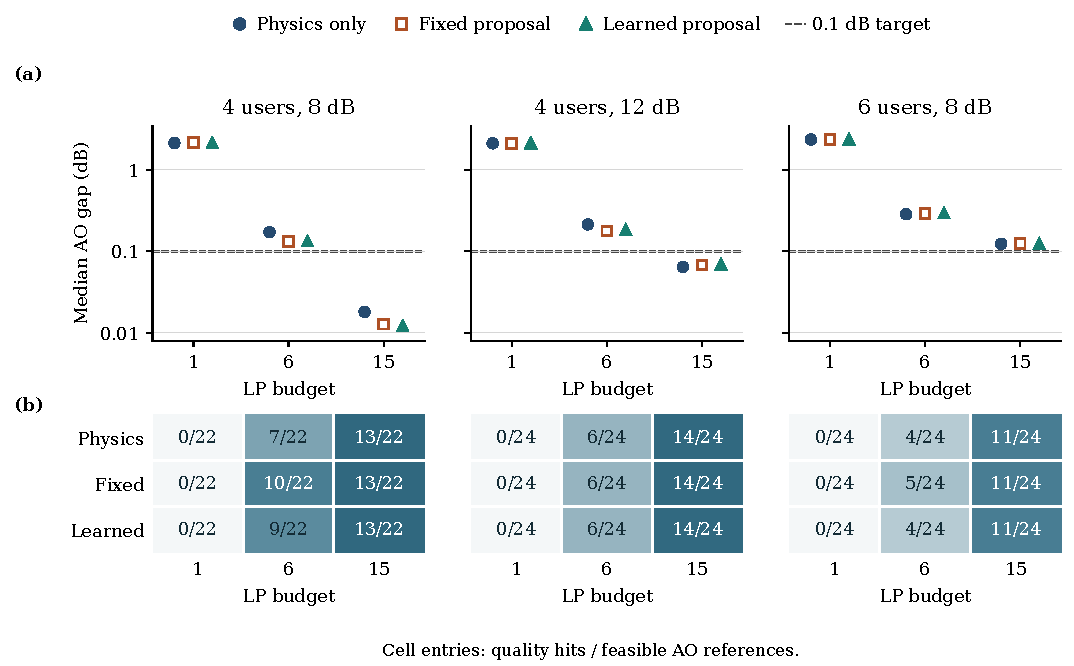
\includegraphics[width=.86\textwidth]{mc-quality.pdf}
\caption{Paired performance across communication loads. (a) Median true-SCNR shortfall from feasible AO at each LP budget. Lower is better. The dashed line marks 0.1 dB. (b) Individual cases within the one-sided 0.1-dB target divided by the number of feasible AO references. A median below the threshold can coexist with a substantial individual miss rate.}
\label{fig:mc}
\end{figure*}

At four users and 8 dB the classical 15-LP design had a median gap of only 0.018 dB, yet it passed the target on 13/22 draws. With six users its median gap reached 0.124 dB and 11/24 draws passed. Across the three conditions the 15-LP result was 38/70 (54.3\%) comparable cases for each variant. This is 38 hits out of 72 attempted cases if both missing references remain in the denominator. At one LP, even the smallest condition-wise median gap exceeded 2 dB and no method met the target. At six LPs, physics-only, fixed-proposal and learned-proposal variants yielded 17, 21 and 19 hits, respectively. Fig.~\ref{fig:mc} shows why a runtime comparison alone would overstate the performance available at low budgets.

\begin{figure*}[t]\centering
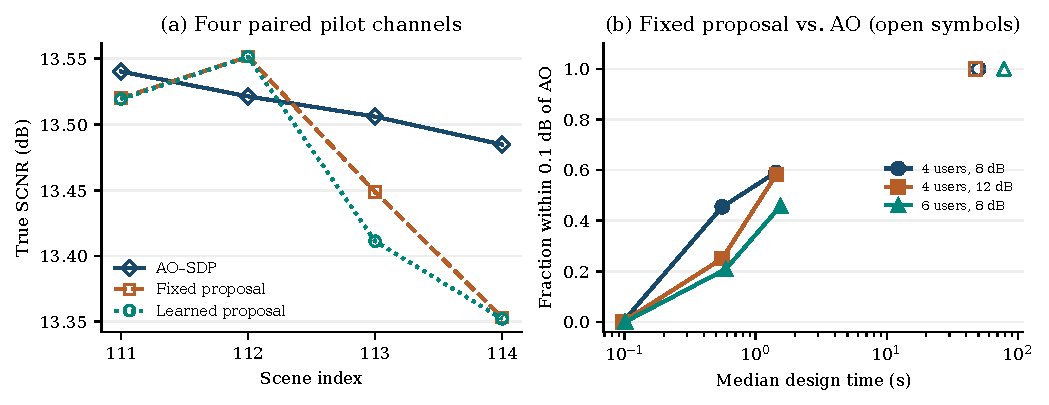
\includegraphics[width=.9\textwidth]{ao-anchor.pdf}
\caption{Measured MATLAB comparisons with the authors' AO--SDP solver. (a) Absolute true SCNR on the four shared pilot scenes at four users and 8 dB, with six LPs for each proposal. (b) Each filled marker is a separate fixed-proposal budget (1, 6 or 15 LPs). The ordinate counts hits among feasible AO pairs; the open marker is AO compared with itself on those pairs. The abscissa is median wall time on all attempted scenes. These are operating points for fixed budgets.}
\label{fig:ao-anchor}\end{figure*}
Figure~\ref{fig:ao-anchor}(a) shows the absolute scale of the comparison. In the larger experiment at four users and 8 dB, the fixed proposal reached the 0.1-dB threshold on 10 of 22 feasible AO pairs at six LPs (0.554 s median), and on 13 of 22 at fifteen LPs (1.426 s median). AO required 50.227 s median across all 24 attempts. Figure~\ref{fig:ao-anchor}(b) displays the increase in cost alongside the increase in success probability.
\subsection{How much of the gain comes from modeling clutter?}
A high output sensing ratio in a clutter-free simulation and a high ratio in a cluttered environment answer different design questions. We separate them with paired interventions on the transmit kernel, receive kernel, and evaluation environment. Each of 12 new seeds (47001--47012) supplies a channel draw for each user count $K\in\{4,8\}$, reused across SINR requirements of 0, 8 and 16 dB. The 72 cases use the same 32 tones, 100 W budget, target coefficient, and underlying clutter environment as the MATLAB benchmark. We use the Python six-allocation fixed-proposal solver throughout this ablation. Each physical return is audited against the original user constraints and total power. The ideal kernel is available for evaluation.

Let $0$ denote the zero cold-clutter map, $\widehat{\mathcal C}$ the estimated map, and $\mathcal C$ the ideal scoring map. In the \emph{joint-aware} design, both transmit and receive updates use $\widehat{\mathcal C}$. In the \emph{blind} design both use $0$, and the returned beams are scored under $\mathcal C$. A third design retains the blind transmit beams and updates only the receiver by \eqref{eq:mvdr} under $\widehat{\mathcal C}$. All three experience the same true clutter and the same $R_{\eta,n}$. Two physical controls change the environment: first we evaluate the blind transceiver with cold scattering absent and $R_{\eta,n}$ retained; then we redesign and evaluate with only spatially white receiver noise, $R_{\eta,n}=\sigma_r^2 I$, using the tutorial's per-tone thermal-noise variance $\sigma_r^2$. The last condition measures a sensing SNR. The target coefficient remains fixed under the benchmark normalization in \eqref{eq:radar}.

\begin{figure*}[t]\centering
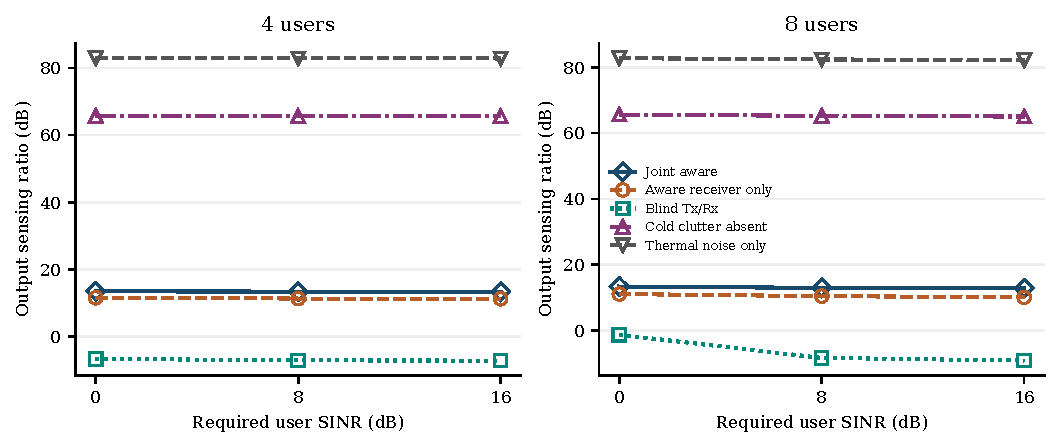
\includegraphics[width=.88\textwidth]{clutter-ablation.pdf}
\caption{Physical clutter removal and clutter-blind design. Each point is the median output sensing ratio over 12 matched channel seeds. The three lower curves share the same physical scattering and additive disturbance. The two upper curves change the physical disturbance. The thermal-only curve retains receiver noise.}\label{fig:cold}
\end{figure*}
At four users and 8 dB, the median true SCNR was $-7.01$ dB with a blind transceiver, 11.37 dB after adapting only its receiver, and 13.44 dB with joint design (Fig.~\ref{fig:cold}). At that operating point, removing cold clutter physically yielded 65.70 dB; thermal noise alone yielded 82.84 dB. For a fixed blind pair, removing cold clutter must increase the score by exactly $10\log_{10}(1+D_c/D_a)$, where $D_c$ and $D_a$ are respectively the cold and additive terms in the denominator of \eqref{eq:ratio}. This identity was checked on every pair. The large absolute levels arise under the tutorial's fixed-power normalization and disturbance scales.

Across all 72 pairs the median gain of joint awareness over blind design was 20.77 dB (95\% seed-cluster bootstrap interval 9.01--21.91 dB). Against the same blind transmitter with an adapted receiver the gain was 2.19 dB (1.99--2.33 dB). The latter comparison isolates the incremental value of redesigning the transmitter when the receiver already has the estimated clutter model. The intervals resample 12 seed clusters, preserving the six operating conditions within each cluster, using 4000 bootstrap resamples. They quantify channel variation within this environment.

\subsection{Conventional transmit directions and communication feasibility}
To isolate the transmit design, maximum-ratio transmission (MRT), zero forcing (ZF) and regularized ZF (RZF) all receive estimated-kernel MVDR filtering. Comparisons of conventional precoders also appear in Wang \emph{et al.}~\cite{wangclutter}; the following power rules target our multitone per-user constraints. Using the normalized channel matrix $G_n$ defined earlier, the direction matrices before column normalization are $G_n$ for MRT and $G_n(G_n^{\mathsf H}G_n+\delta I)^{-1}$ for ZF ($\delta=0$) and RZF ($\delta=0.1$). This fixed regularizer defines the RZF control.

For direction $v_{nk}$ assigned to user $k$, set $b_{ki}=|h_{nk}^{\mathsf H}v_{ni}|^2$ on tone $n$. Define $F_{ki}=\gamma'_{nk}b_{ki}/b_{kk}$ for $i\ne k$, $F_{kk}=0$, and $d_k'=\gamma'_{nk}\sigma_c^2/b_{kk}$. If the spectral radius of $F$ is below one, the minimum user powers are $(I-F)^{-1}d'$, obtained by saturating the QoS inequalities. The inverse is the nonnegative series $\sum_{j\ge0}F^j$, establishing componentwise minimality. If the spectral radius reaches one, a nonnegative left Perron eigenvector applied to $p\ge Fp+d'$ rules out feasibility since $d'>0$. Any surplus system power is distributed equally over tones on their normalized target-steering projections into the user null space. An unavailable fixed-direction design counts as a feasibility failure; its SCNR is omitted.
\begin{figure*}[t]\centering
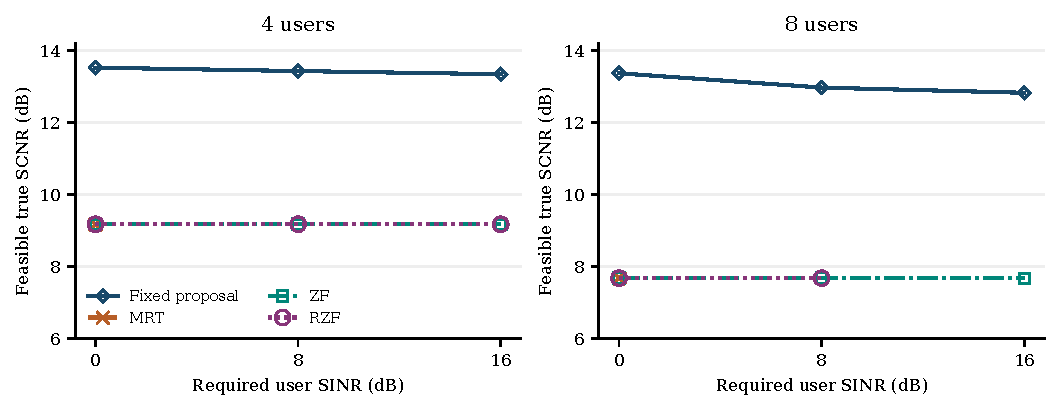
\includegraphics[width=.87\textwidth]{precoder-comparison.pdf}
\caption{True SCNR under identical physical clutter. Each visible point uses all 12 draws for that setting. MRT has feasible points only at 0 dB. RZF is infeasible for all draws at eight users and 16 dB. Similar values among feasible conventional methods reflect their shared null-space sensing beam and power rule.}\label{fig:precoders}
\end{figure*}
Joint design and ZF each returned 72 feasible designs. RZF returned 60 and MRT returned 24. Against ZF, the paired median gain was 4.69 dB (4.63--4.75 dB). Against RZF and MRT, the paired medians were 4.59 and 4.93 dB on their respective feasible subsets. Different subsets prevent interpreting those two medians as a ranking of the conventional methods. The 20.77-dB clutter-awareness result and the 4.69-dB ZF comparison use different controls; neither measures a gain from learning.
\begin{figure*}[t]\centering
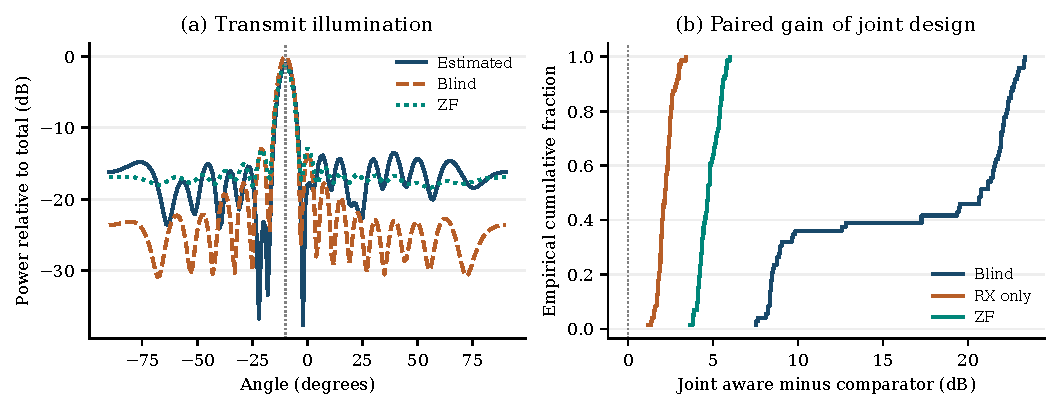
\includegraphics[width=.87\textwidth]{physical-mechanism.pdf}
\caption{(a) Transmit beampattern at four users and 8-dB required SINR, averaged in linear units over 12 channels. At angle $\theta$ we plot $10\log_{10}[\sum_n a_{N_t}(\theta,n)^{\mathsf H}Q_na_{N_t}(\theta,n)/P]$ after averaging; the common reference preserves differences in target illumination. The vertical line marks the target at $-10^\circ$. (b) Empirical distribution of paired true-SCNR gains over all 72 cases. Receive processing and the clutter kernel also determine output SCNR.}\label{fig:pattern}
\end{figure*}

\subsection{Marginal contribution of the learned transmit update}
For each budget and condition, we paired learned and fixed true SCNR on all 24 feasible method pairs. This difference does not require a feasible AO reference. We used 2000 paired bootstrap resamples of channel draws within each setting to obtain percentile intervals for the median. Neither additional timing repetitions nor seed reuse across operating conditions increase the number of independent samples within a setting.

\begin{figure}[t]\centering
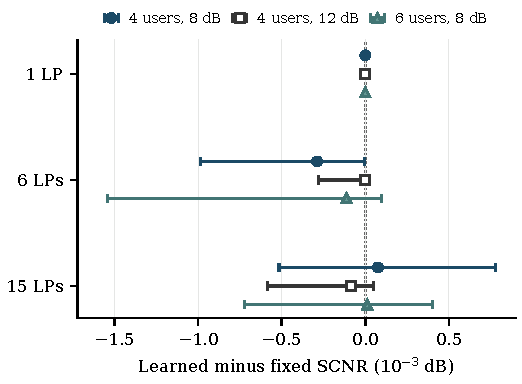
\includegraphics[width=\columnwidth]{learned-gain.pdf}
\caption{Paired median change in true SCNR from enabling learned proposal weights. Whiskers are within-setting 95\% percentile bootstrap intervals from 24 channel pairs. Axis units are thousandths of a dB.}
\label{fig:mc-learn}
\end{figure}

The magnitude of every paired median in Fig.~\ref{fig:mc-learn} was below 0.0003 dB. At four users and 8 dB with six LPs the learned-minus-fixed median was $-0.000288$ dB (bootstrap interval $[-0.000988,-0.000002]$ dB). The fixed proposal alone passed one additional case there and one more at six users and 8 dB. The learned proposal had zero exclusive hits in all nine settings. At fifteen LPs the matched fixed and learned proposals passed exactly the same scenes. The experiment provides no evidence that the frozen policy reduces the LP budget required to meet the specified quality target.

At six LPs the median fixed-proposal design times were 0.554, 0.554 and 0.590 s at the three settings in Table~\ref{tab:mc}, respectively. The corresponding learned-proposal times were 0.554, 0.553 and 0.590 s. Thus the strong latency difference from AO is already present with fixed proposal weights. The effect depends on where the learned update is used. In a separate four-draw development pilot with exact MVDR and the original anchor repair, the learned transmit update improved on its fixed counterpart by a paired median of 0.251 dB, but its recovered design remained 8.40--12.00 dB below AO. The classical 15-LP solver met the quality target on all four development draws. Table~\ref{tab:mc} supplies the larger test of that early observation.
\subsection{Budget sensitivity on independent channels}
A separate Python implementation used the same estimated and ideal clutter maps, SciPy's HiGHS LP backend and a single numerical thread. Both $3\times2$ and $5\times3$ physics-only settings were run on each of 32 new channel draws (seeds 9001--9032), alternating execution order after warm-up. All 64 beam designs passed the feasibility audit. Median true SCNR was 13.437 dB at six solves and 13.463 dB at fifteen. The \emph{paired} median gain was 0.068 dB, with first and third quartiles 0.034 and 0.116 dB. Figure~\ref{fig:gain} shows that the deeper configuration improved true SCNR on 29 draws. The improvement is not monotone in the true score because acceptance operates on the estimated map and the two loop schedules refresh the receiver at different points. Median design times were 0.236 and 0.641 s within this Python experiment. The Python experiment measures budget sensitivity on a separate implementation and set of channels.
\begin{figure}[t]\centering
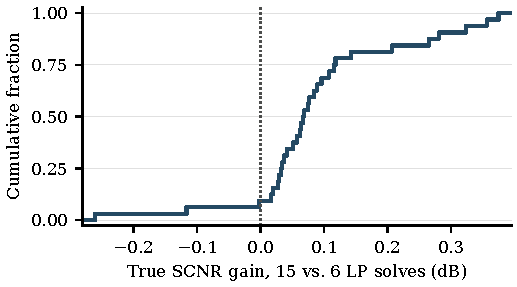
\includegraphics[width=\columnwidth]{budget-gains.pdf}
\caption{Empirical distribution of paired true-SCNR changes over 32 new user-channel draws with the same sensing environment. Each observation compares fifteen with six LP solves using physics-only directions. The dotted line indicates parity.}
\label{fig:gain}
\end{figure}

\subsection{First allocation versus complete solver}
Table~\ref{tab:pd} compares the tied and learned schedules at equal depth. The isolated block uses 12 held-out seeds, three user counts and six thresholds from 0 to 20 dB in 4-dB steps. All three arms share each prepared direction bank and receive filter. The reference for the gap is the optimal estimated-kernel covariance objective on that very bank. This is a stricter control of the learned operation than comparing complete transceiver outputs produced on different banks.
\begin{table}[t]\centering\footnotesize
\caption{Effect of learning power updates. Medians are over matched cases. Hits use a one-sided 0.1-dB tolerance.}\label{tab:pd}
\setlength{\tabcolsep}{4pt}\begin{tabular}{@{}lrrr@{}}\toprule
& Exact LP & Tied & Learned\\\midrule
\multicolumn{4}{l}{First allocation, 216 cases}\\
Bank gap (dB) & 0 & 0.544 & 0.055\\
Bank-quality hits &216&9&126\\
Time incl. recovery and audit (ms)&28.18&7.90&7.97\\
Feasible beams&216&216&216\\\midrule
\multicolumn{4}{l}{Six allocations, 24 cases, only the first varied}\\
Physical true-SCNR gap (dB)&0&0.207&0.314\\
Physical-quality hits&24&9&9\\
Full design time (ms)&390.80&377.50&377.26\\
Feasible beams&24&24&24\\\bottomrule
\end{tabular}\end{table}

On the isolated block, the paired median true-SCNR improvement from learning was 0.215 dB. The mean was 0.704 dB with a 95\% seed-cluster bootstrap interval of $[0.605,0.796]$ dB. Resampling a seed retains its associated loads and thresholds. A certificate changes the latency calculation: requiring the bound in Appendix~\ref{ap:decode} to be within 0.1 dB triggered an exact fallback in 202 of the 216 learned cases and increased median block time to 36.39 ms. The observed 126 quality hits and the small number of certifiable hits answer different questions. An exact reference can measure an error after the experiment even when inexpensive dual information cannot certify that error online.

In the complete solver the comparator is the six-exact-LP fixed-proposal algorithm. The hybrid substitutes only its first solve. Eight held-out seeds at each of three loads and 8 dB give 24 cases. The fixed and learned hybrids each reached the physical true-SCNR target on nine cases. Their mean paired learned-minus-fixed SCNR difference was $-0.018$ dB with a seed-cluster interval of $[-0.061,0.040]$ dB. The first allocation influences both the transmitted power and the directions proposed by its prices. The experiment varies these together, so a final gap cannot be attributed separately to either one. Timings in Table~\ref{tab:pd} use Python and HiGHS on an Intel Xeon Platinum 8573C with one BLAS thread. Methods were interleaved after warm-up, using the within-case median of three repetitions for the block and two for the complete solver. The MATLAB AO times in Table~\ref{tab:mc} belong to a separate benchmark.

\begin{table}[t]\centering\footnotesize
\caption{Effect of truncating the frozen eight-layer power allocator. Each column uses the same 72 new cases. Gaps are relative to the exact first-bank LP.}
\begin{tabular}{lrrrr}\toprule
Layers executed & 2 & 4 & 6 & 8\\\midrule
Tied median gap (dB)&1.811&1.445&0.500&0.323\\
Learned median gap (dB)&1.955&1.594&0.133&0.039\\
Tied hits within 0.1 dB&0&0&0&6\\
Learned hits within 0.1 dB&0&0&25&44\\\bottomrule
\end{tabular}\label{tab:prefix}\end{table}
Table~\ref{tab:prefix} tests the trained schedules on the 72 clutter-ablation cases. At each depth the two methods see the same bank and use the same decoder. Every recovered beam set passed the physical audit. The frozen learned schedule trails the tied control at two and four layers, then achieves the smaller median gap at six and eight. This is a prefix test of the deployed schedule; separately optimizing a schedule at each depth would answer a different question.

\subsection{Scope of the results}
The changed user counts and SINR requirements test transfer with frozen weights under one estimated scattering environment. The design kernel is estimated offline and remains fixed across draws. The current experiment thus measures variability from the communication channels and system load. Testing learning under partial clutter observation would require independent environments and variation in the number and geometry of clutter probes. The fixed-receiver pricing test controls the tightened allocation subproblem. The observed misses concern a different quantity, the final physical-stream SCNR under the true kernel.

\section{Conclusion}
For the considered clutter map, the transmit update admits a useful separation: the receiver determines a marginal target reward and clutter cost for each beam, user multipliers identify costly interference, and scalar powers allocate the shared transmit budget. The resulting pricing test bounds the gap to the unrestricted fixed-receiver covariance design. Physical recovery and a separate audit connect this mathematical guarantee to the beams that would actually be transmitted. In the measured MATLAB benchmark the fifteen-LP solver reduced median design time substantially, although only 38 of 70 comparable cases met the strict 0.1-dB sensing target. Learning was most effective when applied to the first power allocation. The six-allocation comparison identifies the outstanding problem for a learned solver: preserving the local gain as approximate prices influence later directions, while meeting a specified final quality at lower total latency.
\appendices
\section{Receive Update and Transmit Linearization}\label{ap:rx}
For a fixed tone suppress $n$ and write $R=\widehat{\mathcal C}(Q)+R_\eta$. Assume $R_\eta\succ0$, $b\ne0$, and a positive covariance map. For every distortionless $u$, Cauchy--Schwarz gives
\begin{equation}
 1=|(R^{1/2}u)\Hh R^{-1/2}b|^2
 \le (u\Hh Ru)(b\Hh R^{-1}b).
\end{equation}
Equality requires $R^{1/2}u$ to be proportional to $R^{-1/2}b$; the distortionless equality fixes the constant and yields \eqref{eq:mvdr}. Applying this independently at each tone minimizes the denominator of \eqref{eq:ratio} with its numerator fixed. For any Hermitian $Q$, the Frobenius inner product $\langle X,Y\rangle=\tr(X\Hh Y)$ gives
\begin{align}
 u\Hh\widehat{\mathcal C}(Q)u
 &=\vecop(uu\Hh)\Hh\widehat V\vecop(Q)\\
 &=\langle\unvec(\widehat V\Hh\vecop(uu\Hh)),Q\rangle .
\end{align}
Taking the real part gives $\tr(CQ)$ in \eqref{eq:coeff}. For $Q=vv\Hh$ this scalar is nonnegative for every $v$, so $C\succeq0$. In particular, the denominator used in every restricted allocation is positive.
\section{Power Allocation and the Price of an Omitted Beam}\label{ap:price}
\emph{Proposition 1 (exact restricted allocation).} Suppose the fixed bank contains a feasible allocation, $P_s>0$, $d_0>0$, and $s>0$. Then \eqref{eq:lp} attains the maximum fixed-receiver, fixed-bank covariance ratio divided by $s$.
\par\emph{Proof.} Let $D=h\Hh Xh$ be the desired covariance power of one user and $T=h\Hh Qh$ its total received signal power. Its constraint $D\ge\gamma'(T-D+\sigma_c^2)$ is equivalent to $(1+1/\gamma')D-T\ge\sigma_c^2$. Substituting \eqref{eq:dict} and dividing by $P_s\norm h_2^2$ gives the row $Bx\ge d$. The physical power constraint for this tightened problem is $\mathbf1^\top x\le1$ because each dictionary atom has unit norm. For every feasible $x$, $t=(1+c^\top x)^{-1}>0$ and $y=tx$ satisfy \eqref{eq:lp}. Conversely, if $t=0$, the power bound would imply $y=0$, contradicting the equality constraint. Thus every LP solution gives a feasible $x=y/t$ with the same scaled objective. The original power simplex is compact and the objective is continuous, giving attainment.\hfill$\square$

\emph{Proposition 2 (fixed-receiver certificate).} For an optimal restricted primal--dual pair, let $\theta$ be the scaled LP value and $\varepsilon$ the maximum positive pricing violation. Let $v_\infty$ denote the scaled unrestricted covariance optimum with the same $U,P_s,\gamma'$ and the same objective scale $s$. Then
\begin{equation}
 0\le v_\infty-\theta\le\varepsilon .\label{eq:cert}
\end{equation}
\emph{Proof.} With inequality multipliers $\mu,\lambda\ge0$ and equality multiplier $\theta\in\mathbb R$, the maximizing LP has Lagrangian
\begin{align}
 \mathcal L={}&\theta+
 y^\top(\bar\alpha+B^\top\mu-\lambda\mathbf1-\theta c)\notag\\
 &+t(\lambda-d^\top\mu-\theta).
\end{align}
The coefficients of $y,t$ must be nonpositive to bound the supremum over nonnegative variables. Strong LP duality gives the restricted optimum $\theta$. On a new owner-tagged unit vector $v$ at tone $n$, the coefficient of its power equals $v\Hh M_{no}v-\lambda$. Its supremum is the largest eigenvalue of the Hermitian pricing matrix minus $\lambda$. To see why this covers the unrestricted relaxation, spectrally decompose each $X_{nk}$ and the positive semidefinite residual $Q_n-\sum_k X_{nk}$ into nonnegative rank-one terms, assigning the residual owner zero. This gives a finite representation of every unrestricted feasible covariance. Evaluating the same Lagrangian on that representation bounds the primal objective above by $\theta+\varepsilon\mathbf1^\top y$. The equality and $c\ge0$ give $t\le1$, hence $\mathbf1^\top y\le1$. The restricted feasible set is contained in the unrestricted one, giving the other inequality.\hfill$\square$

With zero violation, the current allocation is globally optimal for this tightened, fixed-receiver covariance problem. A finite pricing tolerance gives the additive bound in \eqref{eq:cert}. Numerical eigenvalue and LP residuals matter when the requested tolerance approaches solver precision.
\section{Physical Recovery, Feasibility and Objective Ascent}\label{ap:recover}
\emph{Proposition 3 (feasibility under truncation).} Assume exact covariance feasibility and positive desired powers in \eqref{eq:recover}. Retaining the largest $N_s-K$ nonnegative residual eigenmodes yields beams satisfying the same user thresholds and total power bound. Full covariance recovery holds if $\operatorname{rank}(S_n)\le N_s-K$ on every tone.
\par\emph{Proof.} For each user set $b=X^{1/2}h/\sqrt{h\Hh Xh}$, a unit vector local to this proof. The recovered beam satisfies $ww\Hh=X^{1/2}bb\Hh X^{1/2}\preceq X$ and $|h\Hh w|^2=h\Hh Xh$. The residual $S$ is therefore a sum of positive semidefinite matrices. Its truncation $S_L$ satisfies $0\preceq S_L\preceq S$. The physical covariance $Q_{\rm ph}=\sum_k w_kw_k\Hh+S_L$ obeys $Q_{\rm ph}\preceq Q$. Each user's desired power is preserved and its interference $h\Hh Q_{\rm ph}h-|h\Hh w|^2$ can only decrease. The trace can only decrease as well. The rank condition gives $S_L=S$ and hence equality of covariances.\hfill$\square$

Both target and cold-clutter powers can decrease upon truncation. Their ratio need not improve, which explains the physical design-score acceptance test. In exact arithmetic, with a feasible start and a strictly nondecreasing acceptance rule, the sequence of accepted estimated-kernel scores is nondecreasing. Its numerator is bounded by $P\max_n\kappa_n$ for unit transmit steering vectors and distortionless reception. Its denominator is bounded below by $\sum_n\lambda_{\min}(R_{\eta,n})/\norm{b_n}_2^2>0$, since distortionless reception requires $\norm{u_n}_2\ge1/\norm{b_n}_2$. Thus the objective values of an indefinitely repeated ideal update converge. This proves a statement about scalar values. Joint stationarity would additionally require controlling the transmit approximation, recovery and block optimality in the limit. The measured code uses finite budgets and a relative acceptance tolerance of $10^{-10}$.
\section{Feasible Decoding and an Observable Unfolding Bound}\label{ap:decode}
Flatten the user indices $(n,k)$ into rows $i$. Let $e_i$ denote the coordinate vector of the zero-forcing atom owned by that row and $b_i=(Be_i)_i>0$. Exact zero forcing implies $(Be_i)_j=0$ for $j\ne i$. For any nonnegative candidate $x$, define
\begin{align}
 x_+ &=x+\sum_i e_i[d_i-(Bx)_i]_+/b_i,\\
 x_0 &=\sum_i e_i d_i/b_i .
\end{align}
Then $Bx_+\ge d$ and $Bx_0=d$. Assume $m_0=\mathbf1^\top x_0<1$. If $m_+=\mathbf1^\top x_+\le1$, return $x_+$. Otherwise put $\omega=(1-m_0)/(m_+-m_0)$ and return $(1-\omega)x_0+\omega x_+$. This is a convex combination of two QoS-feasible allocations with unit total mass. These formulas justify the decoder only when the zero-forcing structure and anchor-power condition hold.

For any feasible decoded point of value $r>0$ and prices $z\ge0$, set $q=a-rc+B^\top z$. For every other feasible $x$,
\begin{align}
 (a-rc)^\top x-r
 &\le q^\top x-d^\top z-r\\
 &\le \max(0,\max_j q_j)-d^\top z-r .
\end{align}
Let $e_r$ be the positive part of the final bound. Dividing by $1+c^\top x\ge1$ when the residual is positive gives $\phi(x)-r\le e_r$; a nonpositive residual satisfies the same bound directly. Hence $10\log_{10}(1+e_r/r)$ bounds the attainable improvement in dB for this bank. The bound is computable without the exact LP. A large bound can reflect inaccurate prices even when the returned power allocation is good.

\bibliographystyle{ieeetr}
\bibliography{reference}
\end{document}
